% Options for packages loaded elsewhere
\PassOptionsToPackage{unicode}{hyperref}
\PassOptionsToPackage{hyphens}{url}
\PassOptionsToPackage{dvipsnames,svgnames,x11names}{xcolor}
%
\documentclass[
  letterpaper,
  DIV=11,
  numbers=noendperiod]{scrartcl}

\usepackage{amsmath,amssymb}
\usepackage{lmodern}
\usepackage{setspace}
\usepackage{iftex}
\ifPDFTeX
  \usepackage[T1]{fontenc}
  \usepackage[utf8]{inputenc}
  \usepackage{textcomp} % provide euro and other symbols
\else % if luatex or xetex
  \usepackage{unicode-math}
  \defaultfontfeatures{Scale=MatchLowercase}
  \defaultfontfeatures[\rmfamily]{Ligatures=TeX,Scale=1}
\fi
% Use upquote if available, for straight quotes in verbatim environments
\IfFileExists{upquote.sty}{\usepackage{upquote}}{}
\IfFileExists{microtype.sty}{% use microtype if available
  \usepackage[]{microtype}
  \UseMicrotypeSet[protrusion]{basicmath} % disable protrusion for tt fonts
}{}
\makeatletter
\@ifundefined{KOMAClassName}{% if non-KOMA class
  \IfFileExists{parskip.sty}{%
    \usepackage{parskip}
  }{% else
    \setlength{\parindent}{0pt}
    \setlength{\parskip}{6pt plus 2pt minus 1pt}}
}{% if KOMA class
  \KOMAoptions{parskip=half}}
\makeatother
\usepackage{xcolor}
\setlength{\emergencystretch}{3em} % prevent overfull lines
\setcounter{secnumdepth}{5}
% Make \paragraph and \subparagraph free-standing
\ifx\paragraph\undefined\else
  \let\oldparagraph\paragraph
  \renewcommand{\paragraph}[1]{\oldparagraph{#1}\mbox{}}
\fi
\ifx\subparagraph\undefined\else
  \let\oldsubparagraph\subparagraph
  \renewcommand{\subparagraph}[1]{\oldsubparagraph{#1}\mbox{}}
\fi


\providecommand{\tightlist}{%
  \setlength{\itemsep}{0pt}\setlength{\parskip}{0pt}}\usepackage{longtable,booktabs,array}
\usepackage{calc} % for calculating minipage widths
% Correct order of tables after \paragraph or \subparagraph
\usepackage{etoolbox}
\makeatletter
\patchcmd\longtable{\par}{\if@noskipsec\mbox{}\fi\par}{}{}
\makeatother
% Allow footnotes in longtable head/foot
\IfFileExists{footnotehyper.sty}{\usepackage{footnotehyper}}{\usepackage{footnote}}
\makesavenoteenv{longtable}
\usepackage{graphicx}
\makeatletter
\def\maxwidth{\ifdim\Gin@nat@width>\linewidth\linewidth\else\Gin@nat@width\fi}
\def\maxheight{\ifdim\Gin@nat@height>\textheight\textheight\else\Gin@nat@height\fi}
\makeatother
% Scale images if necessary, so that they will not overflow the page
% margins by default, and it is still possible to overwrite the defaults
% using explicit options in \includegraphics[width, height, ...]{}
\setkeys{Gin}{width=\maxwidth,height=\maxheight,keepaspectratio}
% Set default figure placement to htbp
\makeatletter
\def\fps@figure{htbp}
\makeatother
\newlength{\cslhangindent}
\setlength{\cslhangindent}{1.5em}
\newlength{\csllabelwidth}
\setlength{\csllabelwidth}{3em}
\newlength{\cslentryspacingunit} % times entry-spacing
\setlength{\cslentryspacingunit}{\parskip}
\newenvironment{CSLReferences}[2] % #1 hanging-ident, #2 entry spacing
 {% don't indent paragraphs
  \setlength{\parindent}{0pt}
  % turn on hanging indent if param 1 is 1
  \ifodd #1
  \let\oldpar\par
  \def\par{\hangindent=\cslhangindent\oldpar}
  \fi
  % set entry spacing
  \setlength{\parskip}{#2\cslentryspacingunit}
 }%
 {}
\usepackage{calc}
\newcommand{\CSLBlock}[1]{#1\hfill\break}
\newcommand{\CSLLeftMargin}[1]{\parbox[t]{\csllabelwidth}{#1}}
\newcommand{\CSLRightInline}[1]{\parbox[t]{\linewidth - \csllabelwidth}{#1}\break}
\newcommand{\CSLIndent}[1]{\hspace{\cslhangindent}#1}

\usepackage{lineno}\linenumbers
\KOMAoption{captions}{tableheading}
\makeatletter
\makeatother
\makeatletter
\makeatother
\makeatletter
\@ifpackageloaded{caption}{}{\usepackage{caption}}
\AtBeginDocument{%
\ifdefined\contentsname
  \renewcommand*\contentsname{Table of contents}
\else
  \newcommand\contentsname{Table of contents}
\fi
\ifdefined\listfigurename
  \renewcommand*\listfigurename{List of Figures}
\else
  \newcommand\listfigurename{List of Figures}
\fi
\ifdefined\listtablename
  \renewcommand*\listtablename{List of Tables}
\else
  \newcommand\listtablename{List of Tables}
\fi
\ifdefined\figurename
  \renewcommand*\figurename{Figure}
\else
  \newcommand\figurename{Figure}
\fi
\ifdefined\tablename
  \renewcommand*\tablename{Table}
\else
  \newcommand\tablename{Table}
\fi
}
\@ifpackageloaded{float}{}{\usepackage{float}}
\floatstyle{ruled}
\@ifundefined{c@chapter}{\newfloat{codelisting}{h}{lop}}{\newfloat{codelisting}{h}{lop}[chapter]}
\floatname{codelisting}{Listing}
\newcommand*\listoflistings{\listof{codelisting}{List of Listings}}
\makeatother
\makeatletter
\@ifpackageloaded{caption}{}{\usepackage{caption}}
\@ifpackageloaded{subcaption}{}{\usepackage{subcaption}}
\makeatother
\makeatletter
\@ifpackageloaded{tcolorbox}{}{\usepackage[many]{tcolorbox}}
\makeatother
\makeatletter
\@ifundefined{shadecolor}{\definecolor{shadecolor}{rgb}{.97, .97, .97}}
\makeatother
\makeatletter
\makeatother
\ifLuaTeX
  \usepackage{selnolig}  % disable illegal ligatures
\fi
\IfFileExists{bookmark.sty}{\usepackage{bookmark}}{\usepackage{hyperref}}
\IfFileExists{xurl.sty}{\usepackage{xurl}}{} % add URL line breaks if available
\urlstyle{same} % disable monospaced font for URLs
\hypersetup{
  pdftitle={Size and transparency influence diel vertical migration patterns in copepods.},
  pdfauthor={Alex Barth; Rod Johnson; Joshua Stone},
  colorlinks=true,
  linkcolor={blue},
  filecolor={Maroon},
  citecolor={Blue},
  urlcolor={Blue},
  pdfcreator={LaTeX via pandoc}}

\title{Size and transparency influence diel vertical migration patterns
in copepods.}
\author{Alex Barth \and Rod Johnson \and Joshua Stone}
\date{27 Mar 2023}

\begin{document}
\maketitle
\ifdefined\Shaded\renewenvironment{Shaded}{\begin{tcolorbox}[boxrule=0pt, interior hidden, borderline west={3pt}{0pt}{shadecolor}, enhanced, sharp corners, breakable, frame hidden]}{\end{tcolorbox}}\fi

\setstretch{2}
\hypertarget{abstract}{%
\section{Abstract}\label{abstract}}

Diel vertical migration (DVM) is a widespread phenomenon in aquatic
environments. The primary hypothesis explaining DVM is the visual
predator evasion hypothesis, which suggests that zooplankton migrate to
deeper waters to avoid detection during daylight. However, visual risk
also depends on a copepod's morphology. In this study, we investigate
hypotheses related to morphology and DVM: (H1) size increases visual
risk and will increase DVM depth and (H2) copepod transparency will
reduce visual risk and thus reduce DVM depth. In-situ Copepod images
were collected across several cruises in the Sargasso Sea using an
Underwater Vision Profiler 5. Copepod morphology was characterized from
these images and a dimension reduction approach. The results show a
clear relationship in which larger copepods have a larger DVM signal.
Darker copepods also have a larger DVM signal, however only amongst the
largest group of copepods. This suggests multiple morphological traits
influence copepod DVM behavior.

\hypertarget{scientific-significance-statement}{%
\section{\texorpdfstring{\emph{Scientific Significance
Statement}}{Scientific Significance Statement}}\label{scientific-significance-statement}}

Diel Vertical Migration is a widespread phenomenon across marine and
freshwater systems. The predator evasion hypothesis suggests that DVM
occurs as zooplankton attempt to escape visual predators. Yet, DVM
itself is a costly and risky behavior. Thus, DVM should only occur when
visual risk is high. Several studies have shown that copepod size
influences the magnitude of DVM. However, an individual's visual risk
may include traits beyond simply size. In this study, we utilize an
in-situ imaging tool to reveal how copepod morphological traits
influence DVM. Our findings show that both size and transparency
influence DVM. This finding highlights that DVM is a complex behavior
driven by copepod traits. Furthermore, this study exemplifies the
ability of new technology to draw insights into plankton ecology.

\hypertarget{introduction}{%
\section{Introduction}\label{introduction}}

Diel vertical migration (DVM) is a wide spread phenomena with large
consequences in ocean ecosystems. DVM is the process of pelagic
organisms vertically moving in the water column on a daily basis, often
travelling dozens to hundreds of meters (Bianchi and Mislan 2016). This
large-scale event occurs across many taxa, from plankton to fish
(Brierley 2014). However, DVM is particularly notable in zooplankton
communities, whose migrations contribute substantially to biogeochemical
cycles (Steinberg and Landry 2017; Archibald et al. 2019; Siegel et al.
2023). Zooplankton communities, largely dominated by copepods (Turner
2004), will feed in surface layers of the ocean at night then migrate
into deeper waters during daytime. Through this movement, copepods
actively transport carbon to depth. Additionally, Kelly et al. (2019)
described zooplankton DVM to be a major component of mesopelagic food
webs. Thus to understand pelagic food webs and nutrient cycles, it is
critically important to understand the drivers of DVM.

Predominantly, zooplankton DVM is the movement from deep waters at
daytime to shallower waters at night (Hays 2003; Bianchi and Mislan
2016). The leading explanation for this pattern is the
predator-avoidance hypothesis (Bandara et al. 2021). This hypothesis
posits zooplankton evacuate the sunlit surface to evade visual predators
then ascend at night to feed. However, the massive migration undertaken
by these copepods is energetically expensive (Maas et al. 2018; Robison
et al. 2020). Therefore, the visual predator evasion hypothesis implies
that DVM is a result of visual risk exceeding migration costs. However,
a copepod's visual risk to a visual predator depends on morphological
features (Aksnes and Utne 1997). Notably a copepod's size can increase
visual detection. Several studies have documented that copepod size
influences DVM magnitude (Hays et al. 1994; Aarflot et al. 2019).
Presumably, a copepod's transparency will also influence DVM. Hays et
al. (1994) reported that pigmentation explained variation in DVM
frequency. However, few other studies have investigated this at length.
One barrier to studying a relationship between copepod morphology and
DVM is the difficulty of accurately recording traits.

In-situ imaging tools offer great potential to better describe copepod
DVM. By directly observing copepods, new insights into their behavior
and traits can be resolved (Ohman 2019). For example, Whitmore and Ohman
(2021) used an in-situ imaging device to describe a relationship between
copepod abundance with a particulate field rather than chlorophyll-a.
Such findings are facilitated by the fact imagery data records an
individual's exact position. Additionally, a copepod's true appearance
can be documented whereas net-collected organisms are often physically
deformed or lacking color due to decomposition or preservation. Some
studies have noted a copepod DVM with in-situ imagery data (Pan et al.
2018; Whitmore and Ohman 2021). However, direct tests of DVM-related
hypotheses with such data have not been conducted.

In this study, we utilized in-situ imaging to evaluate how copepod
morphological traits influence patterns. We specifically test the
hypotheses that, (H1) size increases visual risk and will increase DVM
magnitude and (H2) copepod transparency will reduce visual risk and thus
reduce DVM. If these morphologically based hypotheses are true, then the
larger and darker copepods will have the largest DVM signals.

\hypertarget{methods}{%
\section{Methods}\label{methods}}

\hypertarget{ctd-profiles-and-uvp-imaging-of-copepods}{%
\subsection{CTD profiles and UVP imaging of
copepods}\label{ctd-profiles-and-uvp-imaging-of-copepods}}

Data were collected aboard the R/V Atlantic Explorer in collaboration
with the Bermuda Atlantic Time-series Study (BATS) (Steinberg et al.
2001). In-situ images of plankton were acquired using an Underwater
Vision Profiler (UVP5) (Picheral et al. 2010). The original sampling
methodology and instrument specification followed details described in
Barth and Stone (2022). The UVP was attached to the CTD rosette and
deployed regularly on cruises to the Sargasso Sea from June 2019 -
December 2021. Typical monthly cruises included \textasciitilde13
profiles with average descents to 1200m (Supplemental Figure 1). In this
study, we investigated general trends in DVM by pooling together casts
across multiple cruises. This approach is necessitated by the small
sampling volume of the UVP and low abundance of plankton which requires
aggregation of data to resolve trends (Barth and Stone 2022). While
there was some variation between cruises (Supplemental Figure 2), this
oligotrophic system is relatively consistent across seasons.
Additionally, every cruise had an approximately equal number of day and
night casts. Profiles were assigned to be day or night based on locally
calculated nautical dawn and nautical dusk times using the R package
\texttt{suncalc\ 0.5.1}.

The UVP records images of large particles (\textgreater600\(\mu\)m ESD).
However, living particles are not reliably identifiable below 0.9 mm
(Barth and Stone 2022). All recorded images were processed using
Zooprocess (Gorsky et al. 2010), which provides several metrics related
to size, grey value, and shape complexity. These features were then used
to automatically sort images using Ecotaxa (Picheral et al.). All images
were manually verified by the same trained taxonomist. In total, 294,913
images were recorded. Of these, 85.2\% were images of debris or
artefacts. The smallest identified copepod was 0.940mm ESD and the
largest was 5.904mm ESD. Across all casts, copepods were the most common
organism, composing 58.7\% of all identified, living particles. In
total, there were 4151 individual copepods images.

\hypertarget{morphological-grouping}{%
\subsection{Morphological Grouping}\label{morphological-grouping}}

Zooprocess measures and collects several morphologically relevant
parameters. To create relevant groups of copepods, a dimension reduction
approach was used. Similar methods have been successfully utilized to
provide novel insights to marine snow (Trudnowska et al. 2021), copepod
dynamics in the Arctic (Vilgrain et al. 2021), and temporal trends in
phytoplankton communities (Sonnet et al. 2022). First, 18
morphologically relevant parameters were selected to be included in a
principal Components Analysis (PCA), following (Vilgrain et al. 2021).
Parameters can be described as relating to size (e.g.~major axis, feret
diameter, ESD), grey intensity (e.g.~mean grey value at 625nm wavelength
light), shape (e.g.~elongation, symmetry), and shape complexity
(e.g.~fractal dimension). The PCA was weighted by the volume sampled in
a 1-m depth bin for each observation. This approach provides a
correction for the UVP's variable descent speed which can cause
duplicate imaging of individuals. While this phenomena has a minor
impact on overall results (Barth and Stone 2022), we used the weighted
approach to assure that no individual features were overrepresented. All
morphological descriptors were scaled and centered prior to inclusion in
the analysis. The model was constructed using the R package
\texttt{FactoMineR\ 2.7}. principal components were deemed to be
significant if their eigenvalues were greater than 1. This approach
yielded 4 PCs which described 87.3\% of the total variation in
morphological parameters, with 34.5\% and 26.5\% in the first two
components respectively. This four principal component space provides a
``morphospace'' to characterize copepods.

To address our morphology-DVM hypotheses, we constructed discrete
morphological groups based on the first two principal components. Groups
along each of the principal components were defined as low (below 25th
percentile), mid (25th-75th percentile) and high (greater than 75th
percentile). To address the size-dependent hypothesis (H1), groups were
assigned as low, mid, or high along PC1. Then to assess if
color/transparency was a secondary factor (H2), within each PC1 group,
PC2 groups were constructed as low, mid, or high. In total, this created
9 groups (e.g.~Low PC1-Low PC2, Low P1-mid PC2, etc).

\hypertarget{copepod-vertical-structure-dvm}{%
\subsection{Copepod vertical structure \&
DVM}\label{copepod-vertical-structure-dvm}}

\hypertarget{vertical-distribution-of-copepods}{%
\subsubsection{Vertical distribution of
copepods}\label{vertical-distribution-of-copepods}}

Copepods in this system are well documented to undergo DVM (Steinberg et
al. 2000; Schnetzer and Steinberg 2002; Maas et al. 2018). However,
there have not been direct measurements of DVM with in-situ imaging
data. First, to assess which portion of the water column copepods were
utilizing for DVM, we visualized the average vertical structure. The
concentrations of each morphological group (based on PC1 and PC2) were
calculated in 20m depth bins for each UVP profile. These binned-profiles
were then averaged together based on time of day.

\hypertarget{weighted-mean-depth-variability}{%
\subsubsection{Weighted mean depth
variability}\label{weighted-mean-depth-variability}}

Weighted mean depth (WMD) is a common metric to describe vertical
structure and DVM in zooplankton (Ohman et al. 2002; Ohman and Romagnan
2016; Aarflot et al. 2019). However, with in-situ imagery, this approach
presents a few challenges. WMD cannot be calculated individually for
each profile then averaged because each profile had a different descent
depth. Additionally, the small and uneven sampling volume of the UVP can
make single casts too variable to reliably resolve abundance. Yet,
understanding variation around the WMD is necessary to compare DVM
strength across groups. Here, we introduce a depth-bin constrained
bootstrap approach to define WMD with a 95\% confidence interval. To do
this, the concentration of each group, was calculated in 20m depth bins
for each profile. Then all profiles from the same time of day were
`pooled'. This provides a distribution of concentrations in each
depth-bin. Traditional bootstrapping randomly samples, with replacement,
all observations. With vertically structured data however, full random
sampling would bias estimates towards the surface. To avoid this,
samples were ``bin-constrained'' such that for each iteration, a random
observation was sampled within each depth bin, then replaced for the
next iteration. A maximum depth was set to 600m based on observations of
vertical profiles which indicated this to be the maximum point of
day/night differences. This approach effectively created a random
profile by resampling a concentration, \(conc^*\), from each depth bin,
\(d\). This profile then was used to calculate a bootstrapped weighted
mean depth, \(WMD^*\). This was done for each morphological group \(g\),
at each time of day \(t\).

\[WMD^*_{g,t} = \sum_{i}^{N = 60}{\frac{d_i(conc^*_{i,g,t})}{\sum_i^{N = 60}{conc^*_{i,g,t}}}}\]

The distribution of \(WMD^*_{g,t}\) then was used to calculate a
bootstrapped mean and 95\% confidence interval. The 95\% CIs could be
compared between times of day and morphological groups to assess the
strength of DVM. Using PC1 to assess size, the WMD was compared between
the three PC1-groups by percentile level. Then to assess the effect of
transparency the WMD was compared between PC2-groups within each
PC1-grouping. A larger signal of DVM would be evident by a clearly
deeper (non-overlapping 95\% CI) daytime WMD.

\hypertarget{data-availability}{%
\subsection{Data availability}\label{data-availability}}

All data and code are made available via
(https://github.com/TheAlexBarth/DVM\_Migration-Morphology). All
supplemental figures, tables, and analyses are available at
(https://thealexbarth.github.io/DVM\_Migration\_Morphology).

\hypertarget{results}{%
\section{Results}\label{results}}

\hypertarget{morphological-groups}{%
\subsection{Morphological Groups}\label{morphological-groups}}

The PCA revealed four major axis of variability (Figure 1). The first
axis (PC1, 34.23\% of variability) was largely explained by increasing
values related to size, such as perimeter (loading score = 0.927) and
feret diameter (loading score = 0.910). The second axis (PC2, 27.24\% of
variability) can be interpreted as a gradient of transparent to dark
individuals. PC2 was largely anticorrelated with mean grey value (higher
values indicate a more transparent individual) (loading score = -0.920).
As noted in the methods, PC3 and PC4 were both related to the
orientation of the copepod and the appendage visibility respectively
(Supplemental Figure 3).

\begin{figure}

{\centering 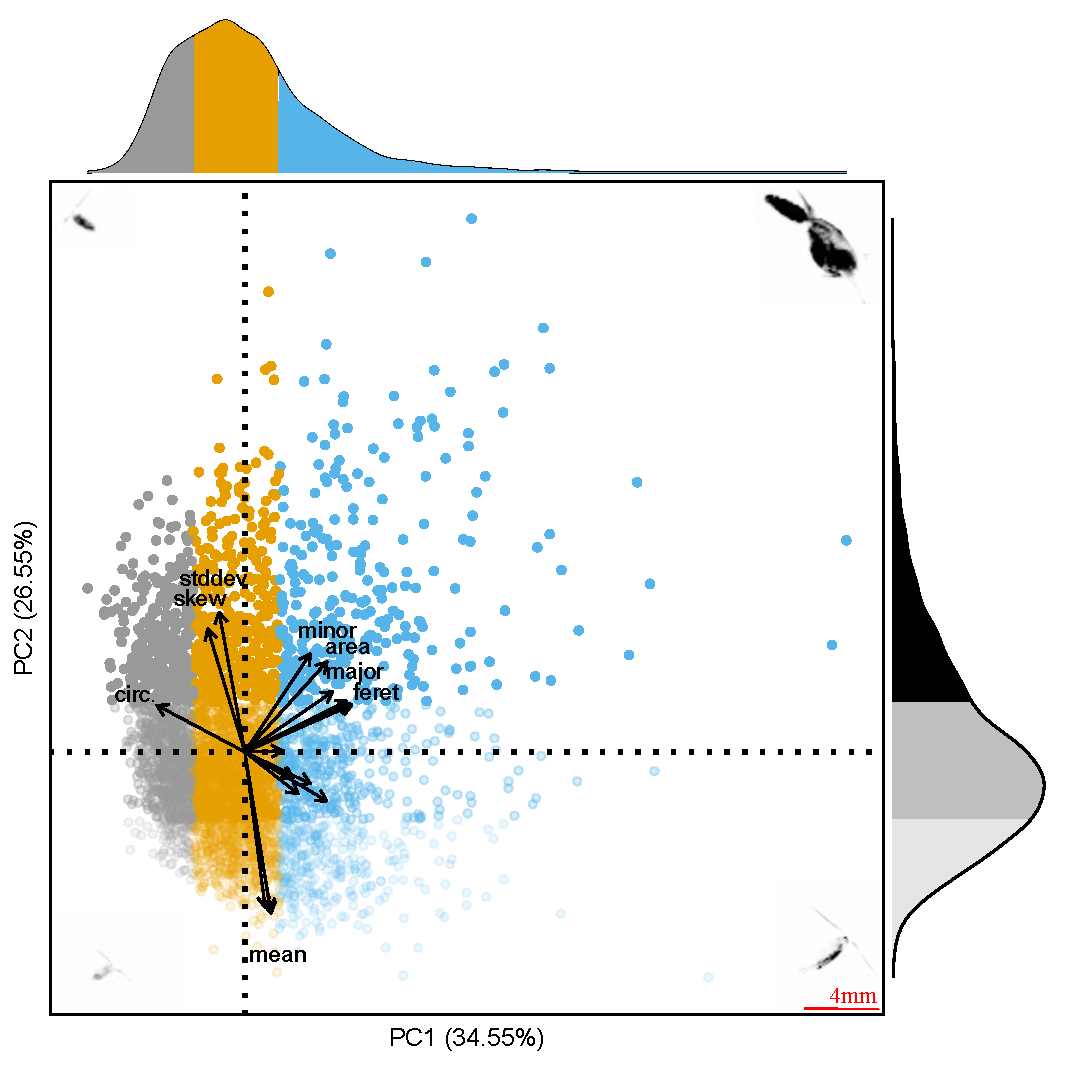
\includegraphics{../media/figure_01.pdf}

}

\caption{First two principal components of the morphospace. Proportion
of variance explained by the two axis is . Each point represents an
individual copepod. The color and transparency of each point
corressponds to the morphological groups based on pecentile along each
axis. Marginal distribution display the proportion of observations in
each group. Representative vignettes of copepods are shown in the
corners corresponding to their place in the morphospace. 4mm scale bar
in the bottom right is shown for the vignettes.}

\end{figure}

The morphological groupings were assigned along PC1 as low, mid and
high. Then along PC2, groups were assigned within each PC1-group (Figure
1). To confirm the morphospace grouping resulted in ecologically
relevant categories, the morphological groups were compared against
known copepod metrics. Across all PC1-groups, there was a clear
difference in feret diameter. The median feret diameter of the low group
was 1.97mm. The median feret diameter of the mid and high groups were
2.84mm and 4.83mm, respectively (Figure 2A). All groups were
significantly different from one another (Dunn Kruskall-Wallace test, p
\textless{} 0.001). PC2 groups as a whole were also significantly
different from one another (Dunn Krustall-wallace test, p \textless{}
0.001). However, within each PC2-group, there was a clear tendency for
larger copepods (high PC1 group) to be more transparent (Figure 2B).

\begin{figure}

{\centering 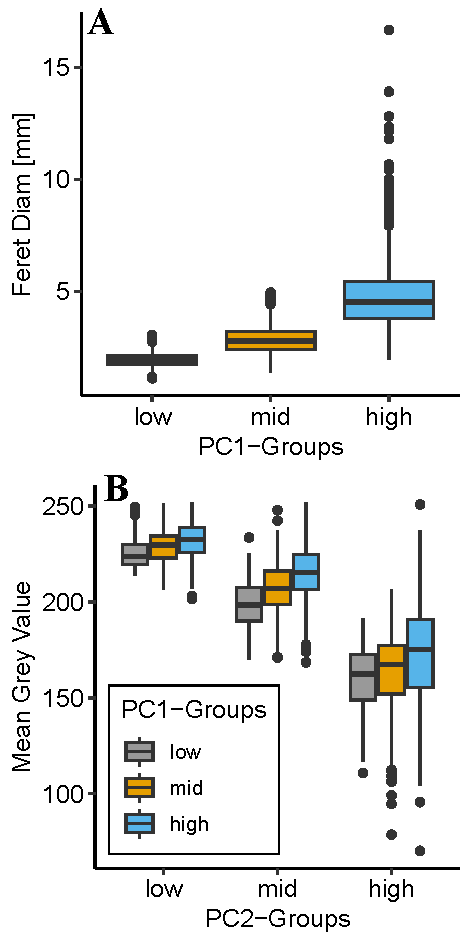
\includegraphics{../media/figure_02.pdf}

}

\caption{Comparison of morphological groups to relevant parameters.
Groups were constructed along principal components with low as below
25th percentile, mid as 25th-50th percentile, and high as above 75th
percentile. (A) PC1 groups are significantly different along feret
diameter and display a clear trend for size. (B) PC2 groups are
significantly different in terms of mean grey value. Note that a low
mean grey value indicates a darker copepod.}

\end{figure}

\hypertarget{vertical-profiles-of-morphological-groups}{%
\subsection{Vertical Profiles of Morphological
Groups}\label{vertical-profiles-of-morphological-groups}}

For all groups, the 20m-binned profiles show a notable structure. While
copepods were observed throughout the mesopelagic (Supplemental Figure
4), the majority of day/night differences were observed above 600m
(Figure 3). For all morphological groups, there was a peak in nighttime
concentration in the lower epipelagic (50m-200m). Similarly, there was a
decrease in average daytime concentration over the same region. This
pattern is particularly apparent for the groups which are mid and high
on both PCs (Figure 3B, C, E, F). Across all groups, both average
daytime and nighttime concentration were low in the upper mesopelagic
(200m-300m). Then, there was a peak in average daytime concentration in
the depth bins in the mid-mesopelagic (400m-600m).

\begin{figure}

{\centering 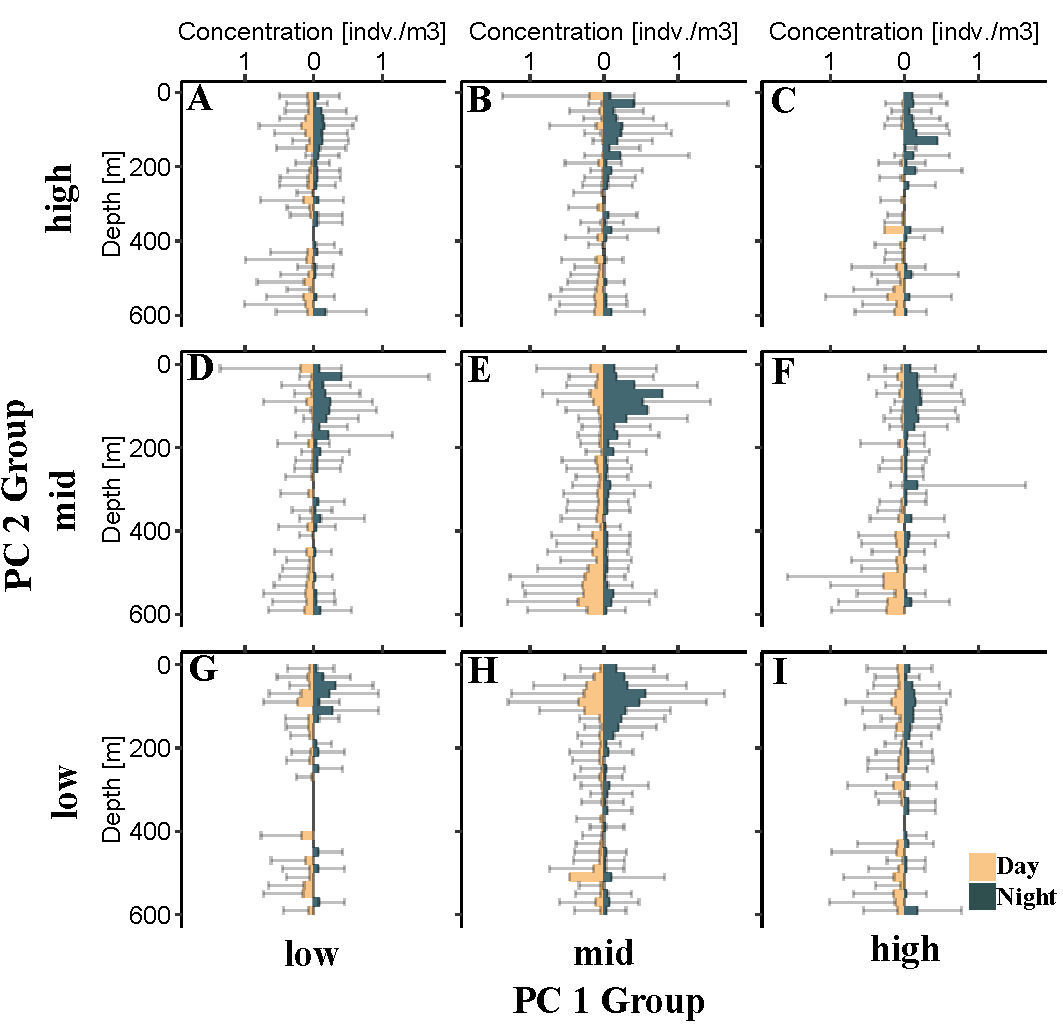
\includegraphics{../media/figure_03.pdf}

}

\caption{Average vertical profile of different copepod morphological
groups. Bars display average concentration in a 20m depth bin. On each
panel, left-side bars (tan) correspond to daytime while right-side
(teal) bars correspond to nighttime. Standard deviation is shown for
each 20m depth bin. Each panel corresponds to a morphological group
along PC1 (size axis) and PC2 (transparency axis). (A) low PC1, high
PC2; (B) mid PC1, high PC2; (C) high PC1, high PC2; (D) low PC1, mid
PC2; (E) mid PC1, mid PC2; (F) high PC1, mid PC2; (G) low PC1, low PC2;
(H) mid PC1, low PC2; (I) high PC1, low PC2}

\end{figure}

\hypertarget{weighted-mean-depth-analysis}{%
\subsection{Weighted mean depth
analysis}\label{weighted-mean-depth-analysis}}

The bin-constrained bootstrap approach provided a direct method to
compare DVM between groups. Size (PC1) had a clear effect on DVM
magnitude. First, for all PC1 groups, daytime WMD 95\% bootstrapped
confidence intervals (95\% CIs) were deeper and non-overlapping with the
nighttime 95\% CIs (Figure 4). This indicates a clear DVM pattern.
However, the differences in day and night CIs varied between
morphological groups. All PC1 groups had a similar, overlapping
nighttime 95\% CI in the lower epipelagic (\textasciitilde145m -
\textasciitilde200m). However, there was a clear difference in the depth
of the daytime 95\% CIs. The small (low PC1) group had the shallowest
95\% CI (235.2m-296.0m). The mid PC1 group's daytime 95\% CI was
slightly deeper (309.0m-347.3m). The large (high PC1) group daytime 95\%
CI was even lower (352.3m-405.0m).

\begin{figure}

{\centering 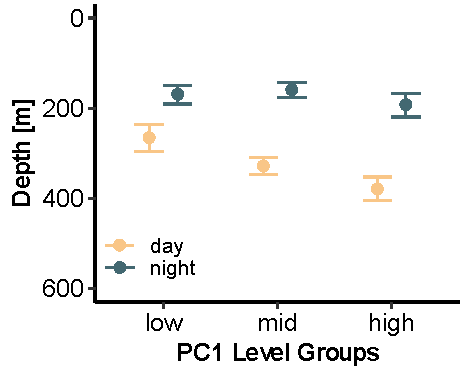
\includegraphics{../media/figure_04.pdf}

}

\caption{Mean bootstrapped weightd mean depth and 95\% confidence
intervals for copepods of different morphological groups. Low, mid, and
high groups correspond to the different percentiles along PC1 from the
morphospace. PC1 largely is explained by size metrics, with higher
scores indicating a larger copepod.}

\end{figure}

When considering the influence of transparency (PC2) on DVM magnitude,
we compared PC2 groups within their PC1 grouping. This approach was
warranted because of the tendency for size to have a slight effect on
transparency (Figure 2). At this level of comparison, there were several
notable trends. For the smaller copepods (low PC1), once the data were
split into PC2 groups, the wider 95\% CIs indicate little to no DVM
signal. Generally, the daytime 95\% CIs and nighttime 95\% CIs are
overlapping or near-overlapping (Figure 5A). With mid sized copepods,
there was a clear DVM signal. However, all PC2 groups appeared to have a
similar DVM magnitude with each group's daytime 95\% CIs overlapping
with each other (Figure 5B). There was a difference in DVM magnitude
across PC2 groups within the largest copepods. The more transparent
copepods (low PC2 group) showed no DVM signal, with a shallow daytime
WMD. However, the darker copepods (mid and high PC2 groups) had deeper
daytime WMDs (Figure 5c).

\begin{figure}

{\centering 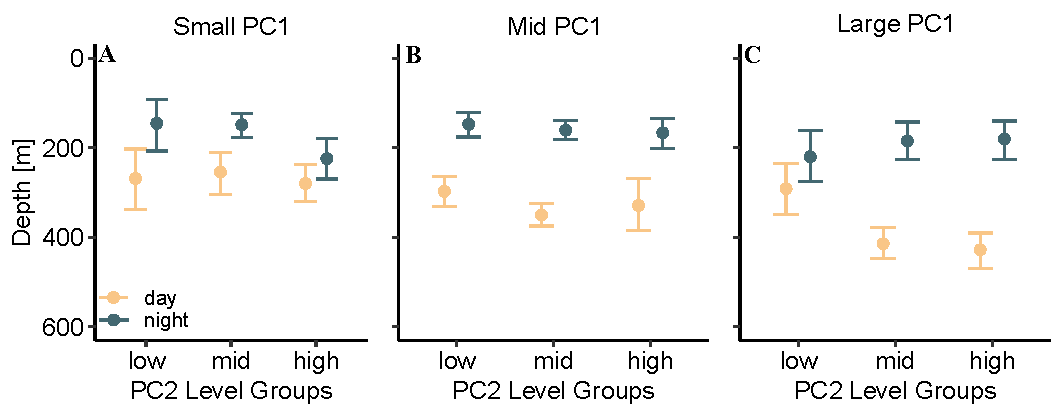
\includegraphics{../media/figure_05.pdf}

}

\caption{Mean bootstrapped weighted mean depth and 95\% confidence
intervals shown by copepod morphological groups along PC2
(transparency). Each panel represents a different size group of copepods
(PC1 groups).}

\end{figure}

\hypertarget{discussion}{%
\section{Discussion}\label{discussion}}

\hypertarget{copepod-morphospace}{%
\subsection{Copepod morphospace}\label{copepod-morphospace}}

In this study, we built on methods for describing morphospaces from
similar in-situ imaging studies (Vilgrain et al. 2021; Trudnowska et al.
2021; Sonnet et al. 2022). The PCA-defined morphospace with the present
data aligns well with the prior applications. Interestingly, the
proportion of variation explained by each axis in the morphospace
defined on Arctic copepods by Vilgrain et al. (2021) is extremely
similar to the morphospace axes in this study. It is possible that this
is an artifact of the similarity of input data. Given the UVP has a
limited range of observable size classes (Picheral et al. 2010), only
copepods above a certain size were fed into both PCAs. Nonetheless, it
is striking that the two morphospaces are similar considering the vastly
different community compositions between the Arctic ocean and
subtropical gyres (Soviadan et al. 2022).

\hypertarget{morphology-and-dvm}{%
\subsection{Morphology and DVM}\label{morphology-and-dvm}}

The pattern of DVM described in this study is consistent with the
general nighttime ascent DVM pattern (Bianchi and Mislan 2016; Bandara
et al. 2021). The average vertical profiles display a clear day/night
difference (Figure 3). In each 20m depth bin, there was large variation,
often exceeding the average concentration. This large variation however,
was expected. There can be considerable variation between UVP estimates
of zooplankton abundance (Barth and Stone 2022). Additionally, in this
study we pooled casts across multiple seasons. Variability in copepod
DVM has been described across seasons (Whitmore and Ohman 2021). While
seasonal variability in DVM is in an interesting question in the
Sargasso Sea, the nature of our dataset did not lend itself to this
investigation. However, despite the need to pool UVP casts across
cruises, the signal of DVM was still observable. Previous studies using
in-situ imaging have also noted a signal of DVM with copepods (Pan et
al. 2018; Whitmore and Ohman 2021). Yet due to small and uneven
sampling, it can be a challenge to quantify DVM using in-situ imaging.
As presented in this paper, bin-constrained bootstrapping offers a
robust method to quantify WMD and investigate DVM hypotheses.

Copepod size had a clear effect in which larger copepods migrated
further. This finding is consistent with several studies which have
documented a size-dependent relationship for copepod DVM (Ohman and
Romagnan 2016; Aarflot et al. 2019; Pinti et al. 2019). Ohman and
Romagnan (2016) noted that moderate-size copepods had the largest
migrations. While this may seem contradictory to the present study, the
difference between study systems needs be taken into account. The
copepods described in the large (high PC1) group had a mean feret
diameter of nearly 5mm. Conversely, in Ohman and Romagnan (2016)'s study
the ``moderate'' copepods ranged from 4mm-6mm. An effect of transparency
on copepod DVM was only observed in the large copepod group. The large
but more transparent copepods (low PC2, high PC1) did not have a
detectable DVM signal. Yet the darker copepods (mid and high PC2) had a
large DVM signal. Hays (2003) described that copepod pigmentation could
explain increased DVM with small (\textless1mm) copepods. The lack of a
transparency effect for the mid- and low PC1 groups in our study is
surprising. One possibility is that the small, transparent copepods were
not well sampled by the UVP (Figure 2). Alternatively, some copepods
which do not migrate may have pigmentation to avoid damage from UV
radiation. The grey-value recorded in UVP-imaged copepods can be
indicative of many features beyond simply pigmentation, notably egg-sacs
and gut contents (Vilgrain et al. 2021). Such characteristics vary much
more between individuals and can have varied influences on DVM (PEARRE
Jr. 2003). Thus the relationship between color and DVM is the result of
a delicate balance of minimizing multiple ecological and biological
risks (Hansson 2004; Hylander et al. 2014). While well documented,
predator avoidance may not always be the primary selective pressure on
copepod traits. For example, if the costs of migration are too large for
some copepods, they will remain near the surface. However, these
copepods then are exposed to UV light and may increase pigmentation to
reduce damage. Overall, our results reveal a complex dynamic between
copepod traits and DVM behavior. Additionally, we show that in-situ
imaging systems can be used to investigate ecological hypotheses.

\hypertarget{sec-references}{%
\subsection*{References}\label{sec-references}}
\addcontentsline{toc}{subsection}{References}

\hypertarget{refs}{}
\begin{CSLReferences}{1}{0}
\leavevmode\vadjust pre{\hypertarget{ref-aarflot2019}{}}%
Aarflot, J. M., D. L. Aksnes, A. F. Opdal, H. R. Skjoldal, and Ø.
Fiksen. 2019. Caught in broad daylight: Topographic constraints of
zooplankton depth distributions. Limnology and Oceanography \textbf{64}:
849--859.
doi:\href{https://doi.org/10.1002/lno.11079}{10.1002/lno.11079}

\leavevmode\vadjust pre{\hypertarget{ref-aksnes1997}{}}%
Aksnes, D. L., and A. C. W. Utne. 1997. A revised model of visual range
in fish. Sarsia \textbf{82}: 137--147.
doi:\href{https://doi.org/10.1080/00364827.1997.10413647}{10.1080/00364827.1997.10413647}

\leavevmode\vadjust pre{\hypertarget{ref-archibald2019}{}}%
Archibald, K. M., D. A. Siegel, and S. C. Doney. 2019. Modeling the
Impact of Zooplankton Diel Vertical Migration on the Carbon Export Flux
of the Biological Pump. Global Biogeochemical Cycles \textbf{33}:
181--199.
doi:\href{https://doi.org/10.1029/2018GB005983}{10.1029/2018GB005983}

\leavevmode\vadjust pre{\hypertarget{ref-bandara2021}{}}%
Bandara, K., Ø. Varpe, L. Wijewardene, V. Tverberg, and K. Eiane. 2021.
Two hundred years of zooplankton vertical migration research. Biological
Reviews \textbf{96}: 1547--1589.
doi:\href{https://doi.org/10.1111/brv.12715}{10.1111/brv.12715}

\leavevmode\vadjust pre{\hypertarget{ref-barth2022}{}}%
Barth, A., and J. Stone. 2022.
\href{https://www.frontiersin.org/articles/10.3389/fmars.2022.898057}{Comparison
of an in situ imaging device and net-based method to study
mesozooplankton communities in an oligotrophic system}. Frontiers in
Marine Science \textbf{9}.

\leavevmode\vadjust pre{\hypertarget{ref-bianchi2016}{}}%
Bianchi, D., and K. a. S. Mislan. 2016. Global patterns of diel vertical
migration times and velocities from acoustic data. Limnology and
Oceanography \textbf{61}: 353--364.
doi:\href{https://doi.org/10.1002/lno.10219}{10.1002/lno.10219}

\leavevmode\vadjust pre{\hypertarget{ref-brierley2014}{}}%
Brierley, A. S. 2014. Diel vertical migration. Current Biology
\textbf{24}: R1074--R1076.
doi:\href{https://doi.org/10.1016/j.cub.2014.08.054}{10.1016/j.cub.2014.08.054}

\leavevmode\vadjust pre{\hypertarget{ref-gorsky2010}{}}%
Gorsky, G., M. D. Ohman, M. Picheral, and others. 2010. Digital
zooplankton image analysis using the ZooScan integrated system. Journal
of Plankton Research \textbf{32}: 285--303.
doi:\href{https://doi.org/10.1093/plankt/fbp124}{10.1093/plankt/fbp124}

\leavevmode\vadjust pre{\hypertarget{ref-hansson2004}{}}%
Hansson, L.-A. 2004. Plasticity in Pigmentation Induced by Conflicting
Threats from Predation and Uv Radiation. Ecology \textbf{85}:
1005--1016. doi:\href{https://doi.org/10.1890/02-0525}{10.1890/02-0525}

\leavevmode\vadjust pre{\hypertarget{ref-hays2003}{}}%
Hays, G. C. 2003. \href{https://doi.org/10.1007/978-94-017-2276-6_18}{A
review of the adaptive significance and ecosystem consequences of
zooplankton diel vertical migrations}. Springer Netherlands. 163--170.

\leavevmode\vadjust pre{\hypertarget{ref-hays1994}{}}%
Hays, G. C., C. A. Proctor, A. W. G. John, and A. J. Warner. 1994.
Interspecific differences in the diel vertical migration of marine
copepods: The implications of size, color, and morphology. Limnology and
Oceanography \textbf{39}: 1621--1629.
doi:\href{https://doi.org/10.4319/lo.1994.39.7.1621}{10.4319/lo.1994.39.7.1621}

\leavevmode\vadjust pre{\hypertarget{ref-hylander2014}{}}%
Hylander, S., J. C. Grenvald, and T. Kiørboe. 2014. Fitness costs and
benefits of ultraviolet radiation exposure in marine pelagic copepods.
Functional Ecology \textbf{28}: 149--158.
doi:\href{https://doi.org/10.1111/1365-2435.12159}{10.1111/1365-2435.12159}

\leavevmode\vadjust pre{\hypertarget{ref-kelly2019}{}}%
Kelly, T. B., P. C. Davison, R. Goericke, M. R. Landry, M. D. Ohman, and
M. R. Stukel. 2019.
\href{https://www.frontiersin.org/articles/10.3389/fmars.2019.00508}{The
importance of mesozooplankton diel vertical migration for sustaining a
mesopelagic food web}. Frontiers in Marine Science \textbf{6}.

\leavevmode\vadjust pre{\hypertarget{ref-maas2018}{}}%
Maas, A. E., L. Blanco-Bercial, A. Lo, A. M. Tarrant, and E.
Timmins-Schiffman. 2018. Variations in copepod proteome and respiration
rate in association with diel vertical migration and circadian cycle.
The Biological Bulletin \textbf{235}: 30--42.
doi:\href{https://doi.org/10.1086/699219}{10.1086/699219}

\leavevmode\vadjust pre{\hypertarget{ref-ohman2019b}{}}%
Ohman, M. D. 2019. A sea of tentacles: optically discernible traits
resolved from planktonic organisms in situ H. Browman {[}ed.{]}. ICES
Journal of Marine Science \textbf{76}: 1959--1972.
doi:\href{https://doi.org/10.1093/icesjms/fsz184}{10.1093/icesjms/fsz184}

\leavevmode\vadjust pre{\hypertarget{ref-ohman2016}{}}%
Ohman, M. D., and J.-B. Romagnan. 2016. Nonlinear effects of body size
and optical attenuation on Diel Vertical Migration by zooplankton.
Limnology and Oceanography \textbf{61}: 765--770.
doi:\href{https://doi.org/10.1002/lno.10251}{10.1002/lno.10251}

\leavevmode\vadjust pre{\hypertarget{ref-ohman2002}{}}%
Ohman, M. D., J. A. Runge, E. G. Durbin, D. B. Field, and B. Niehoff.
2002. On birth and death in the sea. Hydrobiologia \textbf{480}: 55--68.
doi:\href{https://doi.org/10.1023/A:1021228900786}{10.1023/A:1021228900786}

\leavevmode\vadjust pre{\hypertarget{ref-pan2018}{}}%
Pan, J., F. Cheng, and F. Yu. 2018.
\href{http://nopr.niscpr.res.in/handle/123456789/44619}{The diel
vertical migration of zooplankton in the hypoxia area observed by video
plankton recorder}. IJMS Vol.47(07) {[}July 2018{]}.

\leavevmode\vadjust pre{\hypertarget{ref-pearrejr.2003}{}}%
PEARRE Jr., S. 2003. Eat and run? The hunger/satiation hypothesis in
vertical migration: history, evidence and consequences. Biological
Reviews \textbf{78}: 1--79.
doi:\href{https://doi.org/10.1017/S146479310200595X}{10.1017/S146479310200595X}

\leavevmode\vadjust pre{\hypertarget{ref-picheral}{}}%
Picheral, M., S. Colin, and J.-O. Irisson.
\href{http://ecotaxa.obs-vlfr.fr}{EcoTaxa, a tool for the taxonomic
classification of images.}

\leavevmode\vadjust pre{\hypertarget{ref-picheral2010}{}}%
Picheral, M., L. Guidi, L. Stemmann, D. M. Karl, G. Iddaoud, and G.
Gorsky. 2010. The Underwater Vision Profiler 5: An advanced instrument
for high spatial resolution studies of particle size spectra and
zooplankton. Limnology and Oceanography: Methods \textbf{8}: 462--473.
doi:\href{https://doi.org/10.4319/lom.2010.8.462}{10.4319/lom.2010.8.462}

\leavevmode\vadjust pre{\hypertarget{ref-pinti2019}{}}%
Pinti, J., T. Kiørboe, U. H. Thygesen, and A. W. Visser. 2019. Trophic
interactions drive the emergence of diel vertical migration patterns: A
game-theoretic model of copepod communities. Proceedings of the Royal
Society B: Biological Sciences \textbf{286}: 20191645.
doi:\href{https://doi.org/10.1098/rspb.2019.1645}{10.1098/rspb.2019.1645}

\leavevmode\vadjust pre{\hypertarget{ref-robison2020}{}}%
Robison, B. H., R. E. Sherlock, K. R. Reisenbichler, and P. R. McGill.
2020.
\href{https://www.frontiersin.org/articles/10.3389/fmars.2020.00064}{Running
the gauntlet: Assessing the threats to vertical migrators}. Frontiers in
Marine Science \textbf{7}.

\leavevmode\vadjust pre{\hypertarget{ref-schnetzer2002}{}}%
Schnetzer, A., and D. K. Steinberg. 2002. Active transport of
particulate organic carbon and nitrogen by vertically migrating
zooplankton in the Sargasso Sea. Marine Ecology Progress Series
\textbf{234}: 71--84.
doi:\href{https://doi.org/10.3354/meps234071}{10.3354/meps234071}

\leavevmode\vadjust pre{\hypertarget{ref-siegel2023}{}}%
Siegel, D. A., T. DeVries, I. Cetinić, and K. M. Bisson. 2023.
Quantifying the ocean's biological pump and its carbon cycle impacts on
global scales. Annual Review of Marine Science \textbf{15}: null.
doi:\href{https://doi.org/10.1146/annurev-marine-040722-115226}{10.1146/annurev-marine-040722-115226}

\leavevmode\vadjust pre{\hypertarget{ref-sonnet2022}{}}%
Sonnet, V., L. Guidi, C. B. Mouw, G. Puggioni, and S.-D. Ayata. 2022.
Length, width, shape regularity, and chain structure: time series
analysis of phytoplankton morphology from imagery. Limnology and
Oceanography \textbf{67}: 1850--1864.
doi:\href{https://doi.org/10.1002/lno.12171}{10.1002/lno.12171}

\leavevmode\vadjust pre{\hypertarget{ref-soviadan2022}{}}%
Soviadan, Y. D., F. Benedetti, M. C. Brandão, and others. 2022. Patterns
of mesozooplankton community composition and vertical fluxes in the
global ocean. Progress in Oceanography \textbf{200}: 102717.
doi:\href{https://doi.org/10.1016/j.pocean.2021.102717}{10.1016/j.pocean.2021.102717}

\leavevmode\vadjust pre{\hypertarget{ref-steinberg2000}{}}%
Steinberg, D. K., C. A. Carlson, N. R. Bates, S. A. Goldthwait, L. P.
Madin, and A. F. Michaels. 2000. Zooplankton vertical migration and the
active transport of dissolved organic and inorganic carbon in the
Sargasso Sea. Deep Sea Research Part I: Oceanographic Research Papers
\textbf{47}: 137--158.
doi:\href{https://doi.org/10.1016/S0967-0637(99)00052-7}{10.1016/S0967-0637(99)00052-7}

\leavevmode\vadjust pre{\hypertarget{ref-steinberg2001}{}}%
Steinberg, D. K., C. A. Carlson, N. R. Bates, R. J. Johnson, A. F.
Michaels, and A. H. Knap. 2001. Overview of the US JGOFS Bermuda
Atlantic Time-series Study (BATS): a decade-scale look at ocean biology
and biogeochemistry. Deep Sea Research Part II: Topical Studies in
Oceanography \textbf{48}: 1405--1447.
doi:\href{https://doi.org/10.1016/S0967-0645(00)00148-X}{10.1016/S0967-0645(00)00148-X}

\leavevmode\vadjust pre{\hypertarget{ref-steinberg2017}{}}%
Steinberg, D. K., and M. R. Landry. 2017. Zooplankton and the ocean
carbon cycle. Annual Review of Marine Science \textbf{9}: 413--444.
doi:\href{https://doi.org/10.1146/annurev-marine-010814-015924}{10.1146/annurev-marine-010814-015924}

\leavevmode\vadjust pre{\hypertarget{ref-trudnowska2021}{}}%
Trudnowska, E., L. Lacour, M. Ardyna, A. Rogge, J. O. Irisson, A. M.
Waite, M. Babin, and L. Stemmann. 2021. Marine snow morphology
illuminates the evolution of phytoplankton blooms and determines their
subsequent vertical export. Nature Communications \textbf{12}: 2816.
doi:\href{https://doi.org/10.1038/s41467-021-22994-4}{10.1038/s41467-021-22994-4}

\leavevmode\vadjust pre{\hypertarget{ref-turner2004}{}}%
Turner, J. 2004. The importance of small planktonic copepods and their
roles in pelagic marine food webs,.

\leavevmode\vadjust pre{\hypertarget{ref-vilgrain2021}{}}%
Vilgrain, L., F. Maps, M. Picheral, M. Babin, C. Aubry, J.-O. Irisson,
and S.-D. Ayata. 2021. Trait-based approach using in situ copepod images
reveals contrasting ecological patterns across an Arctic ice melt zone.
Limnology and Oceanography \textbf{66}: 1155--1167.
doi:\href{https://doi.org/10.1002/lno.11672}{10.1002/lno.11672}

\leavevmode\vadjust pre{\hypertarget{ref-whitmore2021}{}}%
Whitmore, B. M., and M. D. Ohman. 2021. Zooglider-measured association
of zooplankton with the fine-scale vertical prey field. Limnology and
Oceanography \textbf{66}: 3811--3827.
doi:\href{https://doi.org/10.1002/lno.11920}{10.1002/lno.11920}

\end{CSLReferences}



\end{document}
